\documentclass[preprint,12pt, a4paper, dvipsnames]{elsarticle}

\usepackage{amssymb}

\usepackage{amsthm}
\usepackage{mathtools}

\usepackage{lineno}
\usepackage{listings}

\usepackage{float}

\usepackage{todonotes}
\usepackage{url}

\usepackage{xcolor}

\usepackage{caption}
\usepackage{subcaption}

\definecolor{codegreen}{rgb}{0.25,0.93,0.31}
\definecolor{codegray}{rgb}{0.5,0.5,0.5}
\definecolor{codepurple}{rgb}{0.58,0,0.82}
\definecolor{backcolour}{rgb}{0.95,0.95,0.92}

%
%\lstdefinestyle{mystyle}{
%	backgroundcolor=\color{backcolour},
%	commentstyle=\color{codegreen},
%	keywordstyle=\color{magenta},
%	numberstyle=\tiny\color{codegray},
%	stringstyle=\color{codepurple},
%	basicstyle=\ttfamily\footnotesize,
%	breakatwhitespace=false,
%	breaklines=true,
%	captionpos=b,
%	keepspaces=true,
%	numbers=left,
%	numbersep=5pt,
%	showspaces=false,
%	showstringspaces=false,
%	showtabs=false,
%	tabsize=2
%}
%
%\lstset{style=mystyle}
\lstset{frame=tb,
	language=Python,
	aboveskip=3mm,
	belowskip=3mm,
	showstringspaces=false,
	columns=flexible,
	basicstyle={\small\ttfamily},
	numberstyle=\color{blue},
	keywordstyle=\color{blue},
	commentstyle=\color{PineGreen},
	stringstyle=\color{ForestGreen},
	breaklines=true,
	breakatwhitespace=true,
	tabsize=3,
	escapeinside={@}{@},
	literate=
	{0}{{{\color{red}0}}}1
	{1}{{{\color{red}1}}}1
	{2}{{{\color{red}2}}}1
	{3}{{{\color{red}3}}}1
	{4}{{{\color{red}4}}}1
	{5}{{{\color{red}5}}}1
	{6}{{{\color{red}6}}}1
	{7}{{{\color{red}7}}}1
	{8}{{{\color{red}8}}}1
	{9}{{{\color{red}9}}}1
    {v0}{{{\color{black}v0}}}1 %% we can not style only numeric literals
    {v1}{{{\color{black}v1}}}1
}
\restylefloat{table}

\newcommand{\eg}{{\emph{e.g.\/}}}
\newcommand{\ie}{{\emph{i.e.\/}}}
\newcommand{\ket}[1]{\ensuremath{|#1\rangle}}
\newcommand{\bra}[1]{\ensuremath{\langle#1|}}
\newcommand{\ketbra}[2]{\ensuremath{\ket{#1}\bra{#2}}}
\newcommand{\proj}[1]{\ensuremath{\ketbra{#1}{#1}}}
\newcommand{\braket}[2]{\ensuremath{\langle{#1}|{#2}\rangle}}
\newcommand{\floor}[1]{\ensuremath{\lfloor #1 \rfloor}}
\newcommand{\complexity}[1]{\ensuremath{\mathbf{#1}}}
\newcommand{\new}[1]{ \textcolor{red}{#1} }
\newcommand{\1}{{\rm 1\hspace{-0.9mm}l}}
\newcommand{\Id}{{\rm 1\hspace{-0.9mm}l}}
\newcommand{\connected}{\sim}
\newcommand{\SPAN}{\mathrm{span}}
\newcommand{\Lrm}{\ensuremath{\mathrm{L}}}
\newcommand{\Urm}{\ensuremath{\mathrm{U}}}
\newcommand{\ee}{\ensuremath{\mathrm{e}}}
\newcommand{\dd}{\ensuremath{\mathrm{d}}}
\newcommand{\ii}{\ensuremath{\mathrm{i}}}
\newcommand{\EE}{\mathcal{E}}
\newcommand{\XX}{\mathcal{X}}
\newcommand{\MM}{\mathcal{M}}
\newcommand{\NN}{\mathcal{N}}
\newcommand{\DD}{\mathcal{D}}
\newcommand{\TT}{\mathcal{T}}
\newcommand{\PP}{\mathcal{P}}
\newcommand{\QQ}{\mathcal{Q}}
\renewcommand{\SS}{\mathcal{S}}
\newcommand{\UU}{\mathcal{U}}
\newcommand{\HH}{\mathcal{H}}
\newcommand{\DU}{\mathcal{DU}}
\newcommand{\NOT}{\sigma_x}
\newcommand{\idop}[1][\XX]{\ensuremath{\1_{#1}}}
\newcommand{\diaguni}{\ensuremath{\mathcal{DU}}}
\newcommand{\diag}{\mathrm{diag}}
\newcommand{\tr}{\mathrm{tr}}
\newcommand{\textapprox}{\raisebox{0.5ex}{\texttildelow}}
\journal{SoftwareX}


\usepackage{amsmath}
\newtheorem{theorem}{Theorem}
\newtheorem{proposition}{Proposition}
\newtheorem{remark}{Remark}
\newtheorem{scheme}{Scheme}
\newtheorem{lemma}{Lemma}

\begin{document}

\begin{frontmatter}

\title{PyQBench: a Python library for benchmarking gate-based quantum computers}

\author{Konrad Jałowiecki\corref{cor1}}
\ead{dexter2206@gmail.com}
\cortext[cor1]{Corresponding author}

\author{Paulina Lewandowska}
\author{Profesor Kierownik \L ukasz Pawela}

\address{Institute of Theoretical and Applied Informatics, Polish Academy
	of Sciences, Ba{\l}tycka 5, 44-100 Gliwice, Poland}

\begin{abstract}
We introduce PyQBench, an innovative open-source framework for benchmarking
gate-based quantum computers. PyQBench can benchmark NISQ devices by verifying their capability of
discriminating between two von Neumann measurements. PyQBench offers a simplified, ready-to-use,
command line interface (CLI) for running benchmarks using a predefined parametrized Fourier
family of measurements. For more advanced scenarios, PyQBench offers a way of employing user-defined
measurements instead of predefined ones.

\end{abstract}

\begin{keyword}
%% keywords here, in the form: keyword \sep keyword
Quantum computing \sep
Benchmarking quantum computers \sep
Discrimination of quantum measurements \sep
Discrimination of von Neumann Measurements \sep
Open-source \sep
Python programming

\PACS 03.67.-a \sep 03.67.Lx

\MSC 81P68

\end{keyword}

\end{frontmatter}



\section*{Current code version}
\label{}

\begin{table}[H]
\begin{tabular}{|l|p{6.5cm}|p{6.5cm}|}
\hline
\textbf{Nr.} & \textbf{Code metadata description} & \textbf{Please fill in this
column} \\
\hline
C1 & Current code version & 0.1.0 \\
\hline
C2 & Permanent link to code/repository used for this code version & \url{https://github.com/iitis/PyQBench} \\
\hline
C3 & Code Ocean compute capsule & \todo[inline]{???}\\
\hline
C4 & Legal Code License & Apache License 2.0\\
\hline
C5 & Code versioning system used & git \\
\hline
C6 & Software code languages, tools, and services used & Python, Qiskit, AWS Braket \\
\hline
C7 & Compilation requirements, operating environments \& dependencies &
\texttt{Python >= 3.8}\newline
\texttt{numpy \textapprox= 1.22.0}\newline
\texttt{scipy \textapprox= 1.7.0}\newline
\texttt{pandas \textapprox= 1.5.0}\newline
\texttt{amazon-braket-sdk >= 1.11.1}\newline
\texttt{pydantic \textapprox= 1.9.1}\newline
\texttt{qiskit \textapprox= 0.37.2}\newline
\texttt{mthree \textapprox= 1.1.0}\newline
\texttt{tqdm \textapprox= 4.64.1}\newline
\texttt{pyyaml \textapprox= 6.0}\newline
\texttt{qiskit-braket-provider \textapprox= 0.0.3}\\
\hline
C8 & If available Link to developer documentation/manual &
\url{https://pyqbench.readthedocs.io/en/latest/}\\
\hline
C9 & Support email for questions & \url{dexter2206@gmail.com}\\
\hline
\end{tabular}
\caption{Code metadata (mandatory)}
\label{}
\end{table}


\linenumbers

%% main text

%The permanent link to code/repository or the zip archive should include the
%following requirements:
%
%README.txt and LICENSE.txt.
%
%Source code in a src/ directory, not the root of the repository.
%
%Tag corresponding with the version of the software that is reviewed.
%
%Documentation in the repository in a docs/ directory, and/or READMEs, as
%appropriate.




\section{Motivation and significance}

Noisy Intermediate-Scale Quantum (NISQ)~\cite{preskill} devices are storming the market,
with a wide selection of devices based on different architectures and accompanying software
solutions. Among hardware providers offering public access to their gate--based devices, one could
mention Rigetti, IBM, Oxford Quantum Group, IonQ or Xanadu. Other vendors offer devices operating in
different paradigms. Notably, one could mention D-Wave and their quantum
annealers, or QuEra devices based on neural atoms. \todo[inline]{Expand this list and provide short
description of those architectures}. Most vendors provide their own software stack and
application programming interface for accessing their devices. To name a few, Rigetti's computers
are available through their Forest SDK and PyQuil library and IBM Q computers can be accessed
through Qiskit or IBM Quantum Experience web interface. Some cloud services, like Amazon Braket, offer access to several quantum devices under a unified API. On top of that, several
libraries and frameworks can integrate with different hardware vendors. Examples of such frameworks
include IBM Q's Qiskit or Zapata Computing's Orquestra.

It is well known that NISQ devices have their limitations. The question is to what extent those
devices can perform meaningful computations? To answer this question, one has to devise a
methodology for benchmarking them. For gate--based computers, on which this paper focuses, there
already exist several approaches. \todo[inline]{List the methods} 

\begin{itemize}
	\item several examples of benchmarks -- all our metrics are readily available for devices with two qubits only and circuit depths $< 10$  for all benchmarks it should be possible to execute
	tweaked variants on larger devices when they become available \cite{cornelissen2021scalable}
	\item random benchmarking \cite{liu2022sampling, knill2007randomized, wallman2014randomized} and general overwiev see here \cite{helsen2022general}
	\item MQT Bench: Benchmarking Software and
	Design Automation Tools for Quantum Computing \cite{mqt2022} -- przejebane 
	\item QUARK framework for quantum compjuting application benchmarking for QUBO using D-QAwe ? \cite{quark2022} --  (e. g., a novel QUBO formulation
	of the partial MAX-SAT problem) and benchmark these on
	different infrastructures (e. g., D-Wave and simulation). 
	\item SupermarQ: A Scalable Quantum Benchmark Suite -- Recent works within the quantum computer architecture
	community have taken the first steps towards quantum
	benchmarking. The PPL+2020 [16] suite was evaluated on
	seven superconducting QPUs, focused on characterizing the
	error rates of different operations, and demonstrated the
	time dependence of their performance. The TriQ [17] suite
	was used to perform a cross-platform comparison between
	superconducting and trapped-ion systems and revealed the
	importance of software visibility into the hardware’s native
	gates. However, the scalability of these suites is limited by
	their reliance on circuit simulation to estimate how well the
	QPUs are performing. SupermarQ extends these works by
	introducing a systematic and principled approach to building
	a scalable quantum benchmark suite \cite{supermarq2022}

\end{itemize}
\todo[inline]{What benchmarking techniques are readily available?}

In this paper, we introduce yet another method for benchmarking gate--based devices with a simple
operational interpretation. In our method, we test how well the given device can distinguish between
two von Neumann measurements performed in different bases. We implemented our method in an
open-source Python library called PyQBench. The library supports any device available through Qiskit
library, and thus can be used with providers such as IBM Q or Amazon Braket. Along with the library,
the PyQBench package contains a command line tool for running benchmarks in most common scenarios.




\begin{itemize}
	\item NISQs are becoming widespread and easily available for the general audience
	\item As with any computational technology, there's a need for benchmarking NISQs to assess
	their potential usability.
	\item Our work aims to provide a new benchmarking scheme for gate-based devices.
	\item Why is PyQBench important?
	\begin{itemize}
		\item There exist multiple benchmarking methods already on the market
		\item Most of them have the following drawbacks:
		\begin{itemize}
			\item Their interpretation is not very intuitive (We cannot phrase it like this without
			explaining why it is so)
			\item Hard to use (is this true?)
			\item No libraries are readily available in Python (needs to be checked).
		\end{itemize}
		\item PyQBench is easy to install, it works with any Qiskit backend, and its results are
		easy to understand and interpret.
	\end{itemize}
\end{itemize}


\todo[inline]{In particular, we compile circuits to standard gate sets of the vendor using compiler RECZNEGO?, and we perform experiments across different qubit subsets.}




quantum volume - '' has become the de-facto standard benchmark to quantify the capability of Noisy Intermediate-Scale Quantum (NISQ) devices '' \cite{pelofske2022volume}





Noisy intermediate-scale quantum
(NISQ)~\cite{preskill} devices are currently storming the market. We
have a selection of readily available quantum computers based on different
architectures. Historically, the first widely introduced quantum computing
architecture is D-Wave's quantum annealer.



Additional approaches to quantum computing are currently in development. For
instance we have Ionq's computer based on ion traps and Xanadu's optical
lattices. As they are in prototype versions no access to general public is
provided.

Next, we have computers implementing the gate model of quantum computation.
These are the best potentially developed machines, which can be thought
of as fully quantum computers, by which we understand that the qubits can be in
an entangled state.

Currently one of the main providers of such architectures is Rigetti and its
Quantum Cloud Services platform. The company has
released three generations of QPUs so far: Rigetti 8Q Agave, Rigetti 19Q Acorn
and Rigetti 16Q Aspen-1. The most recent one was deployed in November 2018 and
is a downgrade in terms of number of qubits compared to the previous 19 qubit
one. However, the new chip is reportedly much more robust to noise and the
proposed architecture is much easier to scale up. The new unit is supposed to
serve as a building block for a 128 qubit
system~\footnote{https://medium.com/rigetti/the-rigetti-128-qubit-chip-and-what-it-means-for-quantum-df757d1b71ea}.
As was the case for IBM, Rigetti also provides a \texttt{Python} library,
\texttt{pyquil}~\cite{}, which enables easy access to the machine.

\todo[inline]{co napisac o tym Amazonie, czy nic ?}

\todo[inline]{rysunki architektur}

%
%\begin{figure}[h]
%	\centering
%
%	\includegraphics[width=0.9\linewidth]{aspen.png}
%	\caption{?}
%	\label{fig:aspen}
%\end{figure}


Now the natural question arises: how to construct a good metric of the
computational power of such devices?
Lately, there have emerged propositions from the scientific community on how to
benchmark such devices.

 First let us mention the work by Michielsen
\emph{et.al.}~\cite{michielsen2017benchmarking}. In there the authors study the
IBM-QE device. Their first test is the creation of the entangled state
$\frac{1}{\sqrt{2}} (\ket{01} - \ket{10})$. Next they implement a
two-qubit+two-qubit adder. Another test is an identity operation, realized by an
even number of CNOT operations. Their final test is a quantum error correction
scheme (is it possible with measurement-controlled-operations?). The final
conclusion is that, except for simple circuits, the device fails to return
correct results.

Another, recent approach is utilizing quantum communication protocols in testing
of quantum architectures~\cite{zhukov2019quantum}. Here, the authors decide to
utilize superdense coding and the BB84 quantum cryptography protocol as
benchmarks for the IBM Q devices. They utilize the mutual information of the
transferred bits as a figure of merit for the quantum computer.

Other approaches focus on generative model training. One of these
works~\cite{hamilton2018generative} is aimed at small architectures, up to 5
qubits. Another recently presented is much more
robust~\cite{benedetti2018generative}. The main drawback of both of them is the
level of complication.



The goal of this work is to introduce a new benchmark for Rigetti
architecture...


\label{}
\todo[inline]{
	Introduce the scientific background and the motivation for developing the
	software. - motywacje

	Explain why the software is important, and describe the exact (scientific)
	problem(s) it solves. - czemu ejst wazne, jakie problemy rozwiazuje

	Indicate in what way the software has contributed (or how it will
	contribute in the future) to the process of scientific discovery; if
	available, this is to be supported by citing a research paper using the
	software. - do czego sie to przyczyni w przyszlosci

	Provide a description of the experimental setting (how does the user use
	the software?). - w jaki sposób użytkownik korzysta z oprogramowania?

	Introduce related work in literature (cite or list algorithms used, other
	software etc.). - inne oprogramowania i algorytmy }

!!!!!!!




Suppose we have access to a device performing one of the predefined von Neumann
measurements, $\PP$ or $\QQ$. In PyQBench, we restrict ourselves to discriminating von Neumann measurements.
This is because, unlike other measurement types, they can be implemented on actual hardware. While the $\PP$ and $\QQ$ are known, it is not known which of them is
performed when the device executes. Based on the measurement outcome, you have to guess which
measurement was performed (but you can perform arbitrary unitary operations before and after the
measurement). What is the highest probability of making a correct guess? And what do you have to do
to achieve it? And, most importantly, why would we want to do this?

Suppose that you know a strategy that, for an ideal device, would yield a probability
$p_{\text{succ}}$ of successfully discriminating between two measurements. Will the probability be
the same on an actual physical device? For current, Noisy Intermediate Scale Quantum devices
(NISQs), the answer is: certainly not. However, the error rate that you make when guessing can be
used as a benchmarking metric. PyQBench helps you in organizing such discrimination experiments for
a single qubit system, executing them on real hardware or simulators, and
computing discrimination probabilities based on the measured bitstrings.







\section{Preliminaries and discrimination scheme approach}
This section is divided into two parts.
In Section~\ref{sec:maths}, we introduce the necessary notation and preliminaries needed to understand the concept of PyQBench. Next, in Section~\ref{sec:discrimination-scheme},
we will present a general overview of the discrimination scheme in theoretical terms. We will also mention NISQ devices' limitations and possible practical solutions in the implementation process.

\subsection{Mathematical preliminaries}\label{sec:maths}
Recall that a general quantum
measurement, that is a positive operator valued measure (POVM) $\PP$ is a
collection of positive semidefinite operators $\{E_1, \ldots, E_m \}$ called
\emph{effects}, which sum up to identity, \ie $ \, \, \sum_{i=1}^m E_i = \1$.
In PyQBench, we are interested only in von Neumann measurements, i.e. measurements
for which all the effects are rank-one projectors. Every such measurement can be
parameterized by a unitary matrix $U$ which the effects $\{\proj{u_0}, \ldots, \proj{u_{d-1}}\}$,
are created by taking $\ket{u_i}$ as  $i+1$-th column of the unitary matrix $U$.
We will denote von Neumann measurements described by the matrix $U$ by $\PP_{U}$.

Typically, NISQ devices can only perform measurements in computational $Z$-basis.
To perform an arbitrary von Neumann measurement $\PP_{U}$, one has to first apply $U^\dagger$
to the measured system and then follow with $Z$-basis measurement. Hence, the following two
circuits are equivalent.

\begin{figure}[h!]
	\centering
	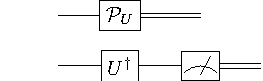
\includegraphics[scale=1.7]{pics/vonneuman}
	\caption{Decomposition of von Neumann measurement}
	\label{fig:vonnneuman}
\end{figure}

Note that the decomposition above is basically a change of basis in which the measurement
is performed.

\subsection{Discrimination scheme}\label{sec:discrimination-scheme}

Without loss of generality, we consider discrimination between a measurement in the computational
Z-basis ($\PP_\Id$), and an alternative measurement performed in the basis $U$
($\PP_U$)\footnote{Explaining why we can consider only Z-basis and alternative measurement is beyond
	the scope of this technical documentation. See \cite{puchala2018strategies} if you are interested in
	the explanation.}. In PyQBench, we operate only on two-level systems, but the discrimination scheme,
described in detail in \cite{puchala2018strategies}, makes no assumptions about the dimensionality.

In general, the discrimination scheme, presented in Fig.\ref{fig:theoretical_scheme}, requires a
second system of the same dimensionality as the measured one. First, the joint system is prepared in
some state $\ket{\psi_0}$. Then, the unknown measurement is performed on the first part of the
system. Based on its outcome $i$, another measurement $\mathcal{P}_{V_i}$ is performed to obtain an
outcome $j$. Finally, if $j=0$ we guess that the performed measurement is $\mathcal{P}_U$, otherwise
we guess that it was $\mathcal{P}_\Id$.

\begin{figure}[h!]
	\centering
	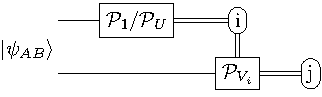
\includegraphics[scale=1.7]{pics/theoretical_scheme}
	\caption{Theoretical  scheme of discrimination  between von Neumann measurements $\PP_{U}$ and $\PP_\Id$. }
	\label{fig:theoretical_scheme}
\end{figure}

\subsubsection{Limitations of NISQ devices and practical discrimination schemes}

Current NISQ devices are unable to perform conditional measurements, which is the biggest
obstacle to implementing our scheme on real hardware. Luckily, we can overcome it by
cleverly adjusting our scheme so that it only uses components available on current devices.
We have two possible choices here: using a postselection or a direct sum
$V_0^\dagger\oplus V_1^\dagger$.

\begin{scheme}(By using postselection)

	The first idea is very simple. Instead of performing a conditional measurement, for each
	measurement $\PP_U, \PP_\Id$ to be discriminated and each choice of $k \in \{0, 1\}$ we run circuit presented in Fig. \ref{fig:postselection}.

	\begin{figure}[h!]
		\centering
		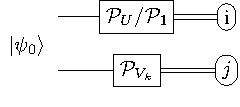
\includegraphics[scale=1.7]{pics/postselection_no_channels}

		\caption{
			Postselection scheme of discrimination between von Neumann measurements $\PP_{U}$ and $\PP_\Id$.
		}\label{fig:postselection}
	\end{figure}

	But now our experiment does not match the previously described scheme, right?
	Yes, unless we discard all the outcomes for which $i\ne k$ (hence the name \emph{postselection},
	we are selecting valid outcomes after the experiment is performed).

	% \begin{scheme}(Postselection)

	% %\begin{figure}[h!]
	% %	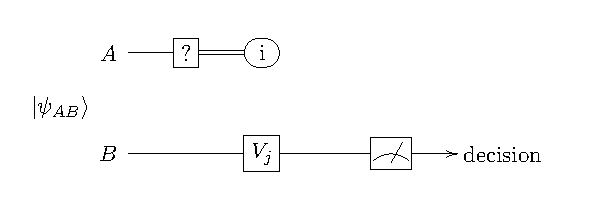
\includegraphics[scale=1.5]{onequbit.pdf}
	% %	\caption{A schematic representation of the setup for distinguishing
	% %		measurements using postselection.}
	% %	\label{postselection}
	% %\end{figure}

	% \begin{enumerate}
	% \item We prepare  the discriminator $\ket{\psi_{0}}$ on bipartite system.
	% \item We perform one of two quantum channels, either $\Phi_{\Id}$ or
	% $\Phi_{U^\dagger}$,  on  the first part of the input state  $\ket{\psi_{0}}$, that means $\left( \Phi \otimes \Id\right)(\proj{\psi_0})$.
	% \item We measure the first part of the input state  $\ket{\psi_{0}}$ and
	% receive an output label $i$.
	% \item
	% Based on Holevo--Helstrom theorem, we perform a conditional binary
	% measurement	$\PP_{V_j}$ and hence, we implement the quantum channel $\Phi_{V_j^\dagger}$ on the second part.
	% \item To calculate the probability of correct discrimination, we include just those cases for which $i = j$.
	% \item We measure the second part of the input state  $\ket{\psi_{0}}$ and make a
	% decision based on received label $j$. If $i=j=0$, then we decide that
	% $\PP_U$ occurs.  If $i=j=1$, we decide that
	% $\PP_{\Id}$ occurs.
	% \end{enumerate}

	More precisely, our experiments can be grouped into classes identified by tuples of the form
	$(\mathcal{Q}, k, i, j)$, where $\mathcal{Q} \in \{\PP_U, \PP_\Id\}$ denotes the chosen measurement.
	We discard all the experiments for which $k \ne i$. Hence, the total number of valid experiments is

	\begin{equation}
	N_\text{total} = \#\{(\QQ, k, i, j): k = i \}.
	\end{equation}

	We now need to count the experiments (among the valid ones) resulting in successful discrimination.
	If we have chosen $\PP_U$, then we guess correctly iff $j=0$. Similarly, for
	$P_\Id$, we guess correctly iff $j=1$. If we define
	\begin{eqnarray}
	N_{\PP_U} &= \#\{(\mathcal{Q}, k, i, j): \mathcal{Q} = \PP_U, k = i, j = 0\}, \\
	N_{\PP_\Id} &= \#\{(\mathcal{Q}, k, i, j): \mathcal{Q} = \PP_\Id, k = i, j = 1\},
	\end{eqnarray}
	then the empirical success probability can be computed as

	\begin{equation}
	p_{\text{succ}}(\PP_{U}, \PP_{\Id}) = \frac{N_{\PP_U} + N_{\PP_\Id}}{N_{\text{total}}}.
	\end{equation}

\end{scheme}

\begin{scheme}(By using direct sum)



	\begin{enumerate}
		\item We prepare the discriminator $\ket{\psi_{0}}$ on bipartite
		system.
		%\item We perform one of two quantum channels, either $\Phi_{\Id}$ or
		%$\Phi_{U^\dagger}$,  on  the first part of the input state  $\ket{\psi_{0}}$, that means $\left(\Phi \otimes \Id\right)(\proj{\psi_0})$.
		\item We apply one of unitary,   either $U^\dagger$ or
		$\Id$, on the first system.
		%\item Based on Holevo--Helstrom theorem, we perform a conditional binary measurement $\PP_{V_j}$, and hence, we implement the direct sum of quantum channels $\Phi_{V_0^\dagger} \oplus \Phi_{V_1^\dagger}$. Observe that   $\Phi_{V_0^\dagger} \oplus \Phi_{V_1^\dagger} = \proj{0} \otimes \Phi_{V_0^\dagger}  + \proj{1} \otimes \Phi_{V_1^\dagger}.  $
		\item We apply direct sum $V_0^\dagger \oplus V_1^\dagger$ on the whole systems.
		\item We measure both systems in computational basis $\Delta$.
		\item We make a decision based on the received label $j$ on the second system. If $j=0$, then we
		decide that $\PP_U$ occurs. Otherwise, we decide that $\PP_{\Id}$ occurs.
	\end{enumerate}

	The schematic representation of this setup is depicted in
	Fig.~\ref{fig:controlled}.
	\begin{figure}[h!]
		\centering
		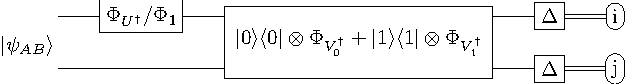
\includegraphics[scale=1.5]{pics/controlled_unitary}

		\caption{ A schematic representation of the setup for distinguishing
			measurements using controlled unitary gate.
		}\label{fig:controlled}
	\end{figure}

	In this scheme, the experiment can be characterized by a pair $(\mathcal{Q}, i,j)$, where $\mathcal{Q} = \{ \PP_{U}, \PP_{\Id} \}$. The number of successful trials for $U$ and $\Id$, respectively, can be written  as
	\begin{eqnarray}
	N_{\PP_U} &= \#\{(\mathcal{Q},  i, j): \mathcal{Q} = \PP_U, j = 0\}, \\
	N_{\PP_\Id} &= \#\{(\mathcal{Q},  i, j): \mathcal{Q} = \PP_\Id, j = 1\}.
	\end{eqnarray}
	Then, the probability of correct discrimination between $\PP_{U} $ and $\PP_\Id$ is given by
	\begin{equation}
	p_{\text{succ}} = \frac{N_{\PP_{U}} + N_{\PP_{\Id}}}{N_{\text{total}}},
	\end{equation}
	where $N_{\text{total}}$ is the number of trials.
\end{scheme}




\subsubsection{Optimal discrimination scheme}


The celebrated result by Helstrom~\cite{helstrom1976quantum} gives the optimal  probability of correct discrimination between two quantum measurements, $\PP$  and $\mathcal{Q}$,
in terms of their distance with the use of the diamond norm
\begin{equation}
p_{\text{succ}}(\PP, \mathcal{Q}) =  \frac12 + \frac14 \| \PP - \mathcal{Q} \|_\diamond,
\end{equation}
where
\begin{equation}
\|\PP\|_\diamond = \max_{\| \ket{\psi}\|_1=1} \| \left(\PP \otimes \1\right) (\proj{\psi}) \|_1.
\end{equation}
The quantum state $\ket{\psi}$ which maximizes the diamond norm is called as discriminator.
Furthermore,  thanks to the proof of the Holevo-Helstrom theorem, it is possible to construct the necessary components  ($\ket{\psi_0}$, $V_0$, $V_1$) to create the optimal discrimination strategy.



 \section{Software description}
 \label{}
 This section is divided into two parts.
 In Section~\ref{sec:sortware-functionalities} we present the details of PyQBench functionality. Next, in Section~\ref{sec:sortware-architecture},
 we will give a general overview of the software architecture.




\subsection{Software Functionalities}\label{sec:sortware-functionalities}


In the scope of this Paper, we aim at  exploring ideas revolving around quantum
gate model-inspired computing devices, and assess their feasibility to
benchmark a modern quantum architectures. The main idea that we have envisioned
for this project is  introducing new concepts of benchmarks for NISQ devices
benchmarking. This project aims to characterize the computing power and
investigate possible practical applications of such devices having access by
Amazon Braket.



\subsection{Software Architecture}\label{sec:sortware-architecture}
PyQBench can be used in two different ways:
\begin{itemize}
\item As a library. This is a more extensible, but also more laborious way of using PyQBench. Most importantly, this way allows for more advanced scripting defining your own measurements scheme.

\item As a CLI tool. This mode of operation trades extensibility for simplicity of usage, as it allows only for running Fourier-discrimination experiments defined with simple YAML input files.
\end{itemize}


\subsubsection{PyQBench as a library}\label{sec:pyqbench-as-library}
This guide introduces basic concepts needed for using PyQBench as a library from a Python script. In particular, we will cover the following topics:
\begin{enumerate}
\item Defining experiment using circuit components.
\item Assembling circuits needed for given benchmarking scheme.
\item Running experiment on simulator or hardware.
\item Obtaining empirical probability of successful discrimination between measurements.
\end{enumerate}

On the conceptual level, every discrimination experiment performed in PyQBench needs the following:
\begin{enumerate}
\item Discriminator, i.e. optimal initial state for the circuit.
\item Unitary $U^\dagger$ defining alternative measurement to be discriminated from the measurement in Z-basis.
\item $V_0^\dagger$ and $V_1^\dagger$, positive and negative parts of optimal measurement from Holevo-Helstrom theorem.
\end{enumerate}
Currently available quantum computers typically cannot start execution from an arbitrary state. Instead, we have to prepare it ourselves. Hence, to execute experiment using postselection scheme, we need an instruction taking to the desired discriminator
and instructions implementing $U^\dagger$, $V_0^\dagger$ and $V_1^\dagger$.

\subsubsection{Example of usage}
In our example, we will use $U =  H$ (the Hadamard gate). To keep us focused on the implementation in PyQBench and not delve too deep into mathematical explanation, we simply provide explicit formulas for discriminator $\ket{\Psi_0} $, $V_0$ and $V_1$, leaving the calculations to the interested reader.

The explicit formula for discriminator in our toy model reads:
\begin{equation}
\ket{\Psi_0} = \frac{1}{\sqrt{2}} (\ket{00} + \ket{11}),
\end{equation}
with corresponding parts of optimal measurement being equal to
\begin{equation}
V_0 =
\left(\begin{array}{cc} \alpha & -\beta\\ \beta & \alpha \end{array}\right),
\end{equation}
and \begin{equation}
V_1 =
\left(\begin{array}{cc} -\beta & \alpha \\ \alpha & \beta \end{array}\right),
\end{equation}
where \begin{equation}
\alpha = \frac{\sqrt{2 - \sqrt{2}}}{2} \cos\left( \frac{3}{8} \pi \right),
\end{equation}
\begin{equation}
\beta  = \frac{\sqrt{2  + \sqrt{2}}}{2} \sin\left( \frac{3}{8} \pi \right).
\end{equation}

As a next step, we need decompose our matrices into actual sequences of gates.
We are lucky, because our discriminator is just a Bell state. Thus, the circuit taking $\ket{00}$ to $\ket{\Phi_0}$ is well known, and comprises Hadamard gate followed by CNOT gate on both qubits.
\begin{figure}[h!]
	\centering
	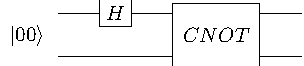
\includegraphics[scale=1.7]{pics/discriminator}
	\caption{Decomposition of the discriminator $\ket{\Phi_0}$. }
	\label{fig:discriminator}
\end{figure}

For $V_0$ and $V_1$ observe that $V_0 = RY\left(\frac{3}{4} \pi \right) $, where $RY$ is rotation gate around the $Y$ axis defined by
\begin{equation}
RY(\theta) =
\left(\begin{array}{cc} \cos\frac{\theta}{2} & -\sin\frac{\theta}{2} \\ \sin\frac{\theta}{2} & \cos\frac{\theta}{2} \end{array}\right).
\end{equation}
To obtain $V_1$  we need only to swap the columns, which is equivalent to following $V_0$ by $X$ matrix, more precisely
\begin{equation}
V_1 =  RY\left(\frac{3}{4} \pi \right) \cdot X.
\end{equation}

Now running the simulation is as simple as invoking functions imported from qbench package.

\todo[inline]{listingi swieca sie na razie jak choinka ale bedziemy kolorki drasowac}
\begin{lstlisting}[language=Python, caption=Simulation benchmark by using postselection]

simulator = Aer.get_backend("aer_simulator")
postselection_result = benchmark_using_postselection(
	backend=simulator,
	target=0,
	ancilla=1,
	state_preparation=state_prep(),
	u_dag=u_dag(),
	v0_dag=v0_dag(),
	v1_dag=v1_dag(),
	num_shots_per_measurement=10000,
)
\end{lstlisting}


\begin{lstlisting}[language=Python, caption=Simulation benchmark by using direct sum]

simulator = Aer.get_backend("aer_simulator")
direct_sum_result = benchmark_using_direct_sum(
backend=simulator,
target=1,
ancilla=2,
state_preparation=state_prep(),
u_dag=u_dag(),
v0_v1_direct_sum_dag=v0_v1_direct_sum_dag(),
num_shots_per_measurement=10000,
)
\end{lstlisting}

\begin{lstlisting}[language=Python, caption=Computation of probability]
p_succ = (2 + np.sqrt(2)) / 4
print(f"Real p_succ = {p_succ}")
print(
f"Postselection: p_succ = {postselection_result}, abs. error = {p_succ - postselection_result}"
)
print(f"Direct sum: p_succ = {direct_sum_result}, abs. error = {p_succ - direct_sum_result}")

\end{lstlisting}


\begin{lstlisting}
Real p_succ = 0.8535533905932737
Postselection: p_succ = 0.8559797193791593, abs. error = -0.0024263287858855564
Direct sum: p_succ = 0.85605, abs. error = -0.0024966094067262468
\end{lstlisting}


\subsubsection{Gaining more control over the benchmarking process}
In the example presented above we used functions that automate the whole process - from the circuit assembly, through running the simulations to interpreting the results. But what if we want more control over some parts of this process? Maybe we want play around with some models? Or maybe we want to run the same experiment on multiple backends and we don’t want them to be assembled over and over again?

 PyQBench provides functions performing:
\begin{enumerate}
\item assembly of circuits needed for experiment, provided the components discussed above
\item interpretation of the obtained measurements
\end{enumerate}
When using these functions, you need to take care of running circuits on some backend yourself, but it gives you unlimited power over the whole process. The difference between such approaches is illustrated on the diagrams below.

When using these functions, you need to take care of running circuits on some backend yourself, but it gives you unlimited power over the whole process. The difference between the two approaches is illustrated on the diagrams below.

\begin{figure}
	\centering
	\begin{subfigure}[b]{\textwidth}
		\centering
		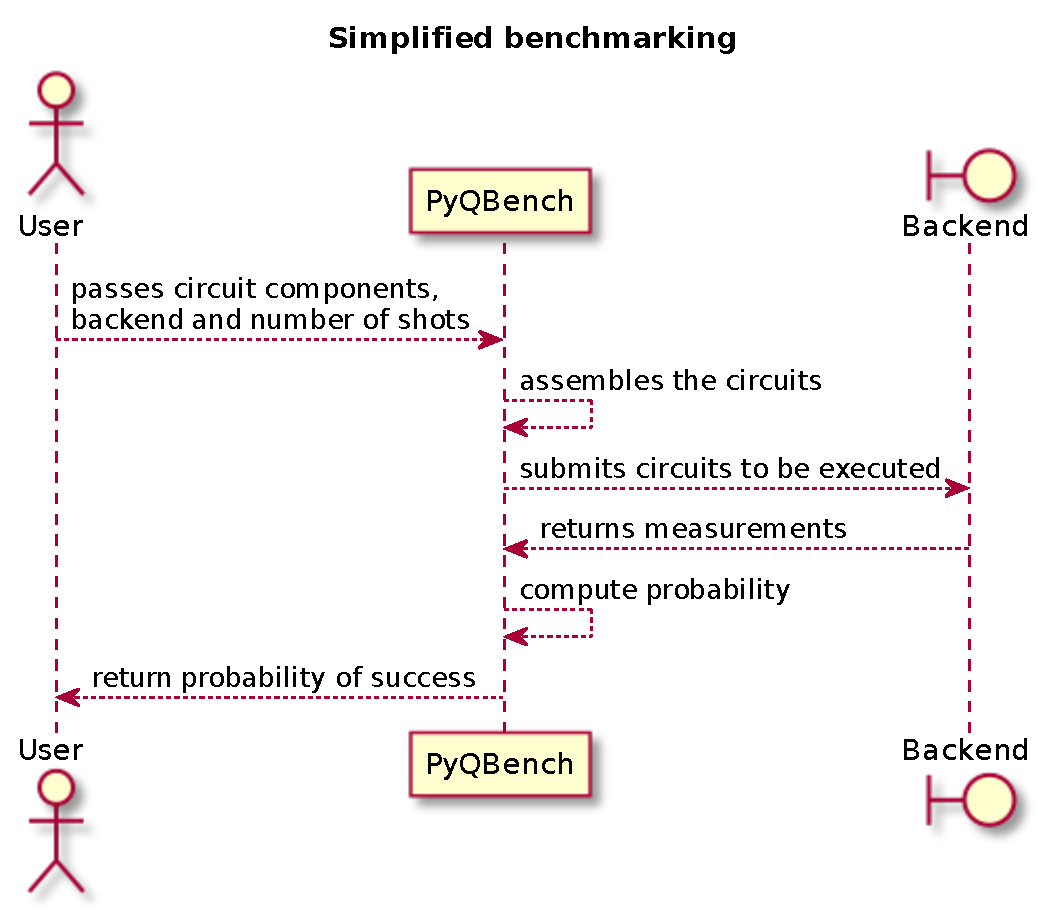
\includegraphics[width=1\textwidth]{pics/scheme1}
%		\caption{$y=x$}
		\label{fig:simplified}
	\end{subfigure}
	\vfill
	\begin{subfigure}[b]{\textwidth}
		\centering
	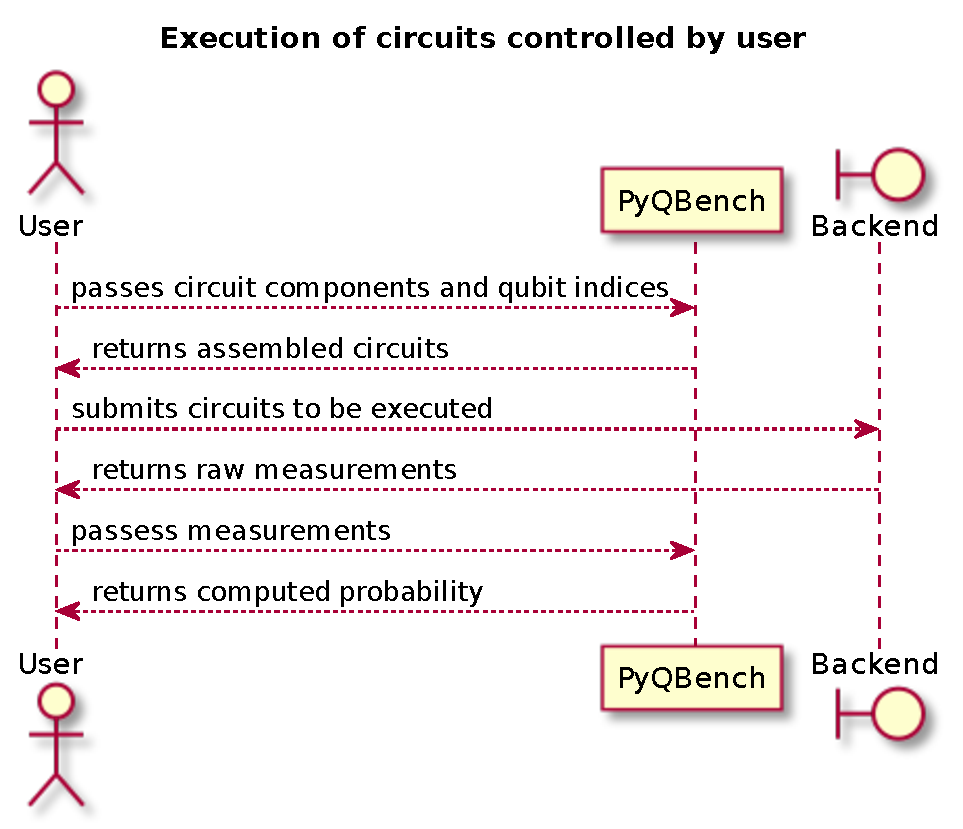
\includegraphics[width=1\textwidth]{pics/scheme2}
%		\caption{$y=3\sin x$}
		\label{fig:execution}
	\end{subfigure}
\end{figure}

\pagebreak


Next, we divide the experiment into two parts:
\begin{enumerate}
	\item Assembling  circuits
	\item Running  circuits
\end{enumerate}


Let us focus only on the postselection case, as the direct sum case is analogous. In addition, we need to import two more functions from PyQBench.




\begin{lstlisting}[language=Python, caption=Assembling circuits]
from qbench.schemes.postselection import (
assemble_postselection_circuits,
compute_probabilities_from_postselection_measurements,
)

circuits = assemble_postselection_circuits(
target=0,
ancilla=1,
state_preparation=state_prep(),
u_dag=u_dag(),
v0_dag=v0_dag(),
v1_dag=v1_dag(),
)

circuits
\end{lstlisting}

%
%\begin{lstlisting}[language=Python, caption=Python example]
%{'id_v0': <qiskit.circuit.quantumcircuit.QuantumCircuit at 0x7f8b1585b9a0>,
%'id_v1': <qiskit.circuit.quantumcircuit.QuantumCircuit at 0x7f8b37fbfa90>,
%'u_v0': <qiskit.circuit.quantumcircuit.QuantumCircuit at 0x7f8b1585bf40>,
%'u_v1': <qiskit.circuit.quantumcircuit.QuantumCircuit at 0x7f8b1585bf10>}
%\end{lstlisting}

Now we only need to run the circuits.
To make things more interesting, we will run a noisy and noiseless simulation of our circuits. We will use the same backend as before, and our noise model will only comprise readout errors on both qubits.

\begin{lstlisting}[language=Python, caption=Noise models]
from qiskit.providers.aer import noise

error = noise.ReadoutError([[0.75, 0.25], [0.8, 0.2]])

noise_model = noise.NoiseModel()
noise_model.add_readout_error(error, [0])
noise_model.add_readout_error(error, [1])

noise_model
\end{lstlisting}

Once we have our noise model ready, we can execute our circuits with and without noise. To this end, we will use Qiskit’s execute function. One caveat is that we have to keep track which measurements correspond to which circuit. We do so by fixing an ordering on the keys in circuits dictionary.

\begin{lstlisting}[language=Python, caption=Running  circuits]
from qiskit import execute

keys_ordering = ["id_v0", "id_v1", "u_v0", "u_v1"]
all_circuits = [circuits[key] for key in keys_ordering]

counts_noisy = (
execute(all_circuits, backend=simulator, noise_model=noise_model, shots=10000).result().get_counts()
)

counts_noiseless = execute(all_circuits, backend=simulator, shots=10000).result().get_counts()


print(f"Noisless counts: {counts_noiseless}")
print(f"Noisy counts: {counts_noisy}")
\end{lstlisting}


%
%Noisless counts: [{'11': 737, '00': 731, '10': 4163, '01': 4369}, {'01': 750, '00': 4217, '10': 716, '11': 4317}, {'01': 740, '10': 693, '00': 4209, '11': 4358}, {'11': 775, '01': 4341, '00': 765, '10': 4119}]
%Noisy counts: [{'01': 1720, '11': 514, '10': 1760, '00': 6006}, {'11': 529, '00': 6025, '10': 1705, '01': 1741}, {'11': 531, '01': 1726, '00': 5956, '10': 1787}, {'01': 1808, '11': 515, '10': 1681, '00': 5996}]



Finally, the only thing left is to compute the success probabilities. We do so by passing bitstring counts to function \\ \texttt{compute\_probabilities\_from\_postselection\_measurements}.


\begin{lstlisting}[language=Python, caption=Computation probability without noise]
prob_succ_noiseless = compute_probabilities_from_postselection_measurements(
id_v0_counts=counts_noiseless[0],
id_v1_counts=counts_noiseless[1],
u_v0_counts=counts_noiseless[2],
u_v1_counts=counts_noiseless[3],
)

print(prob_succ_noiseless)
\end{lstlisting}

\begin{lstlisting}[language=Python, caption=Computation probability including noise]
prob_succ_noisy = compute_probabilities_from_postselection_measurements(
id_v0_counts=counts_noisy[0],
id_v1_counts=counts_noisy[1],
u_v0_counts=counts_noisy[2],
u_v1_counts=counts_noisy[3],
)

print(prob_succ_noisy)
\end{lstlisting}
The success probability is 0.8524401115559386, whereas if we obtain some noise, the succes probability is equal to 0.5017958400693446
As expected, noisy simulations gave us results that are further away from the exact ones.

This concludes introduction to PyQBench library. If you are interested see additoinal usage examples in our examples directory.



\subsubsection{PyQBench as a CLI tool}\label{sec:pyqbench-as-cli}
Using PyQBench as a library allows one to conduct, in principle, arbitrary two-qubit von Neumann measurement experiment. However, as discussed in the previous guide, it requires some amount of boilerplate code.

However, for a Fourier parametrized family of measurements, PyQBench offers a simplified way of performing the experiment using a Command Line Interface (CLI).


\todo[inline]{to be continued }

\section{Discrimination scheme for parameterized Fourier family and implementation}

\subsection{Discrimination scheme}
So far, we only discussed how the discrimination is performed using two different
schemes, assuming that all needed components ($\ket{\psi_0}$, $V_0$, $V_1$) are known. It turned out that the determination of $V_0$ and $V_1$ is a simple task while the discriminator $\ket{\psi_{0}}$ is known. However,
sad to say, determining the analytical form of the discriminator $\ket{\psi_{0}}$
is, in general, NP-hard problem.
We have found the analytical solution of the discrimination scheme for a particular class of von Neumann measurements.


Here,  we will show how all the necessary ingredients look like for
von Neumann measurements defined by the parameterized Fourier family:

\begin{equation}
	U = H
	\left(\begin{array}{cc}1&0\\0&e^{i \phi}\end{array}\right)  H^\dagger,
\end{equation}
where $H$ is the Hadamard matrix of dimension two and $\phi \in [0, 2 \pi)$.
In this case, the optimal input state is Bell state of the form
\begin{equation}
	\ket{\psi_{0}} = \frac{1}{\sqrt{2}} \ket{00} + \ket{11}.
\end{equation}
And, for a given angle  $\phi \in  [0, 2 \pi)$,   the unitaries $V_0$,  $V_1$
have the following form
\begin{equation}
	V_0 = \left(\begin{array}{cc}i \sin\left( \frac{\pi - \phi}{4} \right)&-i
		\cos\left( \frac{\pi - \phi}{4} \right)\\ \cos\left( \frac{\pi -
			\phi}{4}\right)& \sin\left( \frac{\pi - \phi}{4} \right)\end{array}\right),
\end{equation}
\begin{equation}
	V_1 = \left(\begin{array}{cc}-i \cos\left(\frac{\pi - \phi}{4}\right) &i
		\sin\left( \frac{\pi - \phi}{4}\right)\\\sin\left( \frac{\pi - \phi}{4} \right)
		&  \cos\left( \frac{\pi - \phi}{4} \right) \end{array}\right).
\end{equation}
Finally, we have also calculated the theoretical probability of correct discrimination between von Neumann
measurements $\PP_U$ and $\PP_{\Id}$ is given by
\begin{equation}
	p_{\text{succ}}(\PP_{U}, \PP_{\Id}) = \frac{1}{2} + \frac{|1 - e^{i \phi}  |}{4} .
\end{equation}
More details and proofs of the construction's validity   we can find in the \ref{app:optimal-probability} and \ref{app:optimal-strategy}.









\subsection{Implementation}
Here, we will present the results obtained on real devices. For this work we chose IMBQ software. \todo[inline]{tu dokladne informacje o maszynie i rysuneczki}



\section{Impact}
\todo[inline]{OJCIEC WYKAZ SIE, bo trzeba to dobrze sprzedac, nizej tekst z formatki softwarex}
This software has two main contributions.



\textbf{This is the main section of the article and the reviewers weight the
description here appropriately}

Indicate in what way new research questions can be pursued as a result of the
software (if any).

Indicate in what way, and to what extent, the pursuit of existing research
questions is improved (if so).

Indicate in what way the software has changed the daily practice of its users
(if so).

Indicate how widespread the use of the software is within and outside the
intended user group.

Indicate in what way the software is used in commercial settings and/or how it
led to the creation of spin-off companies (if so).

\section{Conclusions}
\label{}

In this study, we develop  a Python library PyQBench, an innovative open-source framework for benchmarking
gate-based quantum computers.


%%%%%%%%%%%%%%
PyQBench can benchmark NISQ devices by verifying their capability of
discriminating between two von Neumann measurements. PyQBench offers a simplified, ready-to-use,
command line interface (CLI) for running benchmarks using a predefined parametrized Fourier
family of measurements. For more advanced scenarios, PyQBench offers a way of employing user-defined
measurements instead of predefined ones.
\section{Conflict of Interest}
No conflict of interest exists: We wish to confirm that there are no known
conflicts of interest associated with this publication and there has been no
significant financial support for this work that could have influenced its out-
come.


\section*{Acknowledgements}


This work is  supported by
the project “Near-term quantum computers Challenges, optimal implementations and applications” under Grant Number POIR.04.04.00-00-17C1/18-00, which is carried out within the Team-Net programme of the Foundation for Polish Science co-financed by the European Union under the European Regional Development Fund.
PL is also a holder of European Union scholarship through the European Social Fund,
grant InterPOWER (POWR.03.05.00-00-Z305).


\begin{thebibliography}{00}
	\bibitem{supermarq} Tomesh, T., Gokhale, P., Omole, V., Ravi, G. S., Smith, K. N., Viszlai, J., ...  Chong, F. T. (2022, April). Supermarq: A scalable quantum benchmark suite. In 2022 IEEE International Symposium on High-Performance Computer Architecture (HPCA) (pp. 587-603). IEEE.
	\bibitem{mqt2022} Quetschlich, N., Burgholzer, L., Wille, R. (2022). MQT Bench: Benchmarking software and design automation tools for quantum computing. arXiv preprint arXiv:2204.13719.
	\bibitem{knill2007randomized} Knill, E., Leibfried, D., Reichle, R., Britton, J., Blakestad, R. B., Jost, J. D., ... Wineland, D. J. (2008). Randomized benchmarking of quantum gates. Physical Review A, 77(1), 012307.
	\bibitem{wallman2014randomized} Wallman, J. J.,  Flammia, S. T. (2014). Randomized benchmarking with confidence. New Journal of Physics, 16(10), 103032.
	\bibitem{helsen2022general} Helsen, J., Roth, I., Onorati, E., Werner, A. H.,  Eisert, J. (2022). General framework for randomized benchmarking. PRX Quantum, 3(2), 020357.
 \bibitem{liu2022sampling} 	Liu, Y., Otten, M., Bassirianjahromi, R., Jiang, L.,  Fefferman, B. (2021). Benchmarking near-term quantum computers via random circuit sampling. arXiv preprint arXiv:2105.05232.
\bibitem{cornelissen2021scalable} Cornelissen, A., Bausch, J.,  Gilyén, A. (2021). Scalable benchmarks for gate-based quantum computers. arXiv preprint arXiv:2104.10698.
\bibitem{quark2022} Finžgar, J. R., Ross, P., Hölscher, L., Klepsch, J.,  Luckow, A. (2022, September). QUARK: A framework for quantum computing application benchmarking. In 2022 IEEE International Conference on Quantum Computing and Engineering (QCE) (pp. 226-237). IEEE.
\bibitem{preskill} Preskill, John. "Quantum Computing in the NISQ era and
beyond." Quantum 2 (2018): 79.
\bibitem{michielsen2017benchmarking} Michielsen, Kristel, et al. "Benchmarking
gate-based quantum computers." Computer Physics Communications 220 (2017):
44-55.
\bibitem{zhukov2019quantum} Zhukov, A. A., et al. "Quantum communication
protocols as a benchmark for programmable quantum computers." Quantum
Information Processing 18.1 (2019): 1-23.
\bibitem{hamilton2018generative} Hamilton, Kathleen E., Eugene F. Dumitrescu,
and Raphael C. Pooser. "Generative model benchmarks for superconducting
qubits." Physical Review A 99.6 (2019): 062323.
\bibitem{benedetti2018generative} Benedetti, Marcello, et al. "A generative
modeling approach for benchmarking and training shallow quantum circuits." npj
Quantum Information 5.1 (2019): 1-9.
\bibitem{puchala2018strategies} Puchała, Zbigniew, et al. "Strategies for
optimal single-shot discrimination of quantum measurements." Physical Review A
98.4 (2018): 042103.
\bibitem{helstrom1976quantum} Helstrom, C. W. (1969). "Quantum detection and estimation theory." Journal of Statistical Physics, 1(2), 231-252.
\bibitem{watrous} Watrous, John (2018). The theory of quantum information. Cambridge university press.
\bibitem{nr} Lewandowska, Paulina and others. The web resource at \url{https://numericalshadow.org/}. Accessed on 2022-10-02.
\bibitem{hausdorff} Hausdorff, Felix. "Der wertvorrat einer bilinearform." Mathematische Zeitschrift 3.1 (1919): 314-316.
\bibitem{toeplitz} Toeplitz, Otto. "Das algebraische Analogon zu einem Satze von Fejér." Mathematische Zeitschrift 2.1 (1918): 187-197.

\bibitem{pelofske2022volume} Pelofske, E., B{\"a}rtschi, A., Eidenbenz, S. (2022). Quantum volume in practice: What users can expect from NISQ devices. arXiv preprint arXiv:2203.03816.
\end{thebibliography}


\todo[inline]{Please add the reference to the software repository if DOI for
software  is available. }

\section*{Current executable software version}
\label{}

Ancillary data table required for sub version of the executable software: (x.1,
x.2 etc.) kindly replace examples in right column with the correct information
about your executables, and leave the left column as it is.

\begin{table}[!h]
\begin{tabular}{|l|p{6.5cm}|p{6.5cm}|}
\hline
\textbf{Nr.} & \textbf{(Executable) software metadata description} &
\textbf{Please fill in this column} \\
\hline
S1 & Current software version & For example 1.1, 2.4 etc. \\
\hline
S2 & Permanent link to executables of this version  & For example:
$https://github.com/combogenomics/$ $DuctApe/releases/tag/DuctApe-0.16.4$ \\
\hline
S3 & Legal Software License & List one of the approved licenses \\
\hline
S4 & Computing platforms/Operating Systems & For example Android, BSD, iOS,
Linux, OS X, Microsoft Windows, Unix-like , IBM z/OS, distributed/web based
etc. \\
\hline
S5 & Installation requirements \& dependencies & \\
\hline
S6 & If available, link to user manual - if formally published include a
reference to the publication in the reference list & For example:
$http://mozart.github.io/documentation/$ \\
\hline
S7 & Support email for questions & \\
\hline
\end{tabular}
\caption{Software metadata (optional)}
\label{}
\end{table}

\appendix
\section{Mathematical preliminaries} \label{app:preliminaries}

Let $M_{d_1,d_2}$ be the set of all matrices of dimension $d_1 \times d_2$ over
the field $\mathbb{C}$. For  simplicity, square matrices will be denoted by
$M_d$.
%The subset of $M_d$ consisting of Hermitian matrices of dimension $d$
%will  be  denoted  by $\HH_d$,  while  the  set  of  positive semidefinite
%matrices of dimension $d$ by $\HH_d^+$.
By $\Omega_d$, we will denote the set of quantum states, that is
positive semidefinite operators having trace equal to one.
The subset of $M_d$ consisting of unitary matrices will be denoted
by $\UU_d$, while its subgroup of diagonal unitary operators will be denoted by
$\DD \UU_d$.
%An operator $A = \left( a_{i,j}\right)_{i,j} \in M_d$ is said to be a stochastic matrix if $a_{i,j} \ge 0$   and $\sum_{i} a_{i,j} = 1$, whereas an operator $A = \left( a_{i,j}\right)_{i,j} \in M_d$ is said to be a double stochastic matrix if $A$ is a stochastic matrix and $\sum_{j} a_{i,j} = 1$.


We will also need a linear mapping transforming $M_{d_1}$ into
$M_{d_2}$, which will be denoted
\begin{equation}
\Phi: M_{d_1 } \rightarrow M_{d_2}.
\end{equation}
There
exists a bijection between the set of linear mappings $\Phi$ and the set of matrices $M_{d_1d_2}$,  known as the Choi-Jamio{\l}kowski isomorphism.
For a given linear mapping $\Phi$ the corresponding Choi operator $J(\Phi)$ is explicitly written as
\begin{equation}
J(\Phi) \coloneqq \sum_{i,j=0}^{d- 1} \Phi(\ketbra{i}{j}) \otimes \ketbra{i}{j}. \end{equation}

We introduce a special subset of all mappings $\Phi$, called quantum channels, which are completely positive
and trace preserving (CPTP).
In this work we will consider a special class of quantum channels, called unitary channels.  A
channel
$\Phi_{U}$ is said to be a unitary channel if it has the following form $\Phi_U(\cdot) = U \cdot U^\dagger$ for any $U \in
\UU_d$.


The action of
von Neumann measurement $\PP_{U}$ on some state $\rho \in \Omega_d$ can be
seen as  a measure-and-prepare quantum channel as follows \begin{equation}
\PP_{U} : \rho \rightarrow \sum_{i=0}^{d-1} \bra{u_i} \rho \ket{u_i} \proj{i}.
\end{equation}
Moreover, observe that each von Neumann measuement $\PP_{U}$ poses a  composition of a unitary channel $\Phi_{U^\dagger}$ and the maximally dephasing channel $\Delta$, that means $\PP_{U} = \Delta \circ \Phi_{U^\dagger}$.

We need to also briefly discuss about the distance between unitary channels and von Neumann measurements. From \cite[Theorem 1]{puchala2018strategies}, the distance between measurements $\PP_U$ and
$\PP_\Id$ ie equal to
\begin{equation}
\|\PP_U - \PP_\Id\|_\diamond = \min_{E \in \diaguni_d} \|\Phi_{UE} -
\Phi_\Id\|_\diamond,
\end{equation} whereas to express the distance between unitary channels, we need to introduce the notion of numerical range. The set \begin{equation}
W(A) =\{\bra{x}A\ket{x}: \ket{x} \in
\mathbb{C}^d, \;
\;\braket{x}{x}=1\}.
\end{equation}
is called numerical range of  a matrix $A \in M_d$.
The detailed properties of the numerical range and its generalizations we can see on the website~\cite{nr}.
Due to the definition of $W(A)$, the distance between two unitary channels $\Phi_{U} $ and $\Phi_\Id$
can be written as
\begin{equation}
\| \Phi_U  - \Phi_{\1} \|_\diamond = 2 \sqrt{1-\nu^2},
\end{equation}
where $\nu = \min_{x \in W(U^\dagger)} |x|  $.


\section{Optimal probability} \label{app:optimal-probability}


Let us focus on single-qubit von Neumann measurements $\PP_\1$ and $\PP_U$.
Assume that the unitary matrix $U$ is of the form
\begin{equation}
U = H
\left(\begin{array}{cc}1&0\\0&e^{i \phi}\end{array}\right)  H^\dagger
\end{equation}
%\begin{equation}
%U = H \diag (1, \ee^{\ii \phi}) H^\dagger,
%\end{equation}
where $H$ is the Hadamard matrix of dimension two and $\phi \in [0, 2 \pi)$.
In this section we present theoretical probability of correct
discrimination between these measurements. To do that, we will present an auxiliary lemma.
\begin{lemma}\label{lemma:min-e-optimal}
	Let $U = H \diag(1, e^{i \phi}) H^\dagger$, $\phi \in [0, 2\pi)$ and	let
	$\Phi_U$ and $\Phi_\Id$ be two unitary channels. Then, the following equation holds
	\begin{equation}
	\min_{E \in \diaguni_2} \|\Phi_{UE} -
	\Phi_\Id\|_\diamond = \|\Phi_{U} -
	\Phi_\Id\|_\diamond,
	\end{equation}
\end{lemma}

\begin{proof} Recall that the distance between two unitary channels is given by
	$
	\| \Phi_U  - \Phi_{\1} \|_\diamond = 2 \sqrt{1-\nu^2},
	$
	where $\nu = \min_{x \in W(U^\dagger)} |x|  $ for any $U \in \mathcal{U}_d$.
	For $U = H
	\left(\begin{array}{cc}1&0\\0&e^{i \phi}\end{array}\right)  H^\dagger$ the readers briefly observe that  $\nu^2 = 1 - \frac{|1 - e^{-i \phi} |^2 }{4} = 1 - \frac{|1 - e^{i \phi} |^2 }{4}$. So,
	\begin{equation}
	\|  \Phi_U  - \Phi_{\1} \|_\diamond = | 1 - e^{i \phi} |.
	\end{equation}
	It implies that it is enough to prove  \begin{equation}
	\min_{E \in \diaguni_2} \|\Phi_{UE} -
	\Phi_\Id\|_\diamond  = | 1 - e^{i \phi} |.
	\end{equation}
	%		It implies that we can prove  equivalently  the following condition
	%		\begin{equation}
	%		\max_{E \in \diaguni_2 } \nu_{UE} = \nu_U
	%		\end{equation}
	This condition is equivalent to show
	\begin{equation}
	\max_{E \in \diaguni_2 } \nu_{E} = \frac{|1 + e^{i \phi} | }{2},
	\end{equation}
	where $\nu_E = \min_{x \in W(U^\dagger E)} |x|. $

	%	For simplify notation, let 	$ \nu \coloneqq \max_{E \in \diaguni_2 } \nu_{E} $.
	The celebrated Hausdorf-T{\"o}plitz theorem~\cite{hausdorff, toeplitz} states that
	$W(A)$ of any matrix $A \in M_d$ is a convex set, and therefore we have
	\begin{equation}
	W(A) = \{ \tr(A \rho): \rho \in \Omega_d\}.
	\end{equation}
	So, we can assume that
	\begin{equation}
	\min_{\ket{x} \in \mathbb{C}^2:   \proj{x} = 1} |\bra{x}U^\dagger\ket{x}| =
	\min_{\rho \in \Omega_2} |\tr(U^\dagger\rho)|.
	\end{equation}
	Then, we have
	\begin{equation}
	\max_{E \in \diaguni_2 } \nu_{E}  = \max_{E \in \diaguni_2 }  \min_{\rho \in
		\Omega_2} \left| \tr \left( \rho U E \right) \right|.
	\end{equation}
	For that, our task is reduced to show that
	\begin{equation}
	\forall_{E \in \diaguni_2} \,\, | \tr \left(\rho U E\right) | \le \max_{E \in \diaguni_2 } \nu_{E}.
	\end{equation}



	Let us define $E = \left(\begin{array}{cc}E_0&0\\0&E_1\end{array}\right)  $
	and take $\rho =
	\left(\begin{array}{cc}\frac{1}{2}&0\\0&\frac{1}{2}\end{array}\right) $.
	From spectral theorem, let us decompose $U$ as
	\begin{equation}
	U= \lambda_0 \ketbra{x_0}{x_0} + \lambda_1 \ketbra{x_1}{x_1},
	\end{equation}
	where  for eigenvalue $\lambda_0 = 1$, the corresponding
	eigenvector is
	of the form $\ket{x_0} = \left[\begin{array}{c}\frac{1}{\sqrt{2}}\\\frac{1}{\sqrt{2}}\end{array}\right]
	$,
	whereas for  $\lambda_1= e^{i \phi}$ we have $\ket{x_1} = \left[\begin{array}{c}\frac{1}{\sqrt{2}}\\-\frac{1}{\sqrt{2}}\end{array}\right]
	$.
	Then, we have
	\begin{equation}
	\begin{split}
	& \forall E \in \diaguni_2 \,\,\, | \tr (\rho U E) | = \frac{1}{2}  \left| \tr \left(
	H \diag(1, e^{i\phi}) H^\dagger E \right) \right| =  \\ &
	\frac{1}{2} \left| \tr\left((   \proj{x_0} +e^{i \phi}\proj{x_1} ) E \right)
	\right|  =
	\frac{1}{2} \left|  \bra{x_0} E \ket{x_0} +  e^{i \phi}\bra{x_1} E \ket{x_1}
	\right| = \\&
	\frac{1}{2} \left| \frac{E_0 + E_1}{2} + e^{i \phi } \frac{E_0+E_1}{2} \right|
	=
	\frac{\left| 1+ e^{i \phi } \right|}{2} \left| \frac{E_0 + E_1}{2} \right| \le
	\max_{E \in \diaguni_2 } \nu_{E},
	\end{split}
	\end{equation}
	which completes the proof.
\end{proof}



\begin{theorem}\label{th:probability}
	The optimal probability of correct discrimination between von Neumann
	measurements $\PP_U$ and $\PP_{\Id}$ for $U = H \diag(1, e^{i \phi}) H^\dagger$,
	where $\phi \in [0, 2\pi)$ is given by
	\begin{equation}
	p_{\text{succ}}(\PP_{U}, \PP_{\Id}) = \frac{1}{2} + \frac{|1 - e^{i \phi}  |}{4} .
	\end{equation}
\end{theorem}



\begin{proof}
	From Holevo-Helstrom theorem, we obtain
	\begin{equation}
	p_{\text{succ}}(\PP_{U}, \PP_{\Id}) = \frac{1}{2} + \frac{1}{4} \| \PP_{U} - \PP_{\Id} \|_\diamond.
	\end{equation}
	From~\cite[Theorem 1]{puchala2018strategies}, we have
	\begin{equation}
	\|\PP_U - \PP_\Id\|_\diamond = \min_{E \in \diaguni_d} \|\Phi_{UE} -
	\Phi_\Id\|_\diamond.
	\end{equation}
	From Lemma~\ref{lemma:min-e-optimal},  we know that for
	$U =  H \diag(1, e^{i \phi}) H^\dagger$,  it also holds that
	\begin{equation}
	\min_{E \in \diaguni_2} \|\Phi_{UE} -
	\Phi_\Id\|_\diamond = \|\Phi_{U} -
	\Phi_\Id\|_\diamond,
	\end{equation} which is exactly equal to
	\begin{equation}
	\|\Phi_{U} -
	\Phi_\Id\|_\diamond = 2\sqrt{1 - \nu^2} = |1-e^{i   \phi }|.
	\end{equation}
	%	Finally, we obtain that
	%	\begin{equation}
	%	\| \PP_{U} - \PP_{\Id} \|_\diamond =  |1-e^{i   \phi }|.
	%	\end{equation}
	It implies that
	\begin{equation}
	p_{\text{succ}}(\PP_{U}, \PP_{\Id}) = \frac{1}{2} + \frac{|1-e^{i \phi}|}{4},
	\end{equation} which completes the proof.
\end{proof}

\section{Optimal discrimination strategy} \label{app:optimal-strategy}


In this Appendix we create the optimal
theoretical strategy of  discrimination between $\PP_{U}$ and $\PP_{\Id}$.
To indicate the optimal strategy, we will present two propositions. The first one is concentrated around the discriminator as the optimal input state of discrimination strategy, whereas the second one describes the optimal final measurement.


\begin{proposition}\label{prop-discrim}
	Consider the problem of discrimination between von Neumann measurements $\PP_U$
	and $\PP_\1$, $U = H\diag(1, e^{i \phi}) H^\dagger $ and $\phi \in [0,
	2\pi)$.  The  discriminator has the form
	\begin{equation}
	\ket{\psi_{0}} = \frac{1}{\sqrt{2}} |\Id_2 \rangle \rangle.
	\end{equation}
\end{proposition}

\begin{proof}
	Let $U = H\diag(1, e^{i \phi}) H^\dagger, \phi \in [0,
	2\pi)$ be decomposed as
	\begin{equation}
	U= \lambda_1 \ketbra{x_1}{x_1} + \lambda_2 \ketbra{x_1}{x_2},
	\end{equation}
	where  for eigenvalue $\lambda_1 = 1$, the corresponding
	eigenvector is
	of the form $\ket{x_1} = \left[\begin{array}{c}\frac{1}{\sqrt{2}}\\\frac{1}{\sqrt{2}}\end{array}\right]
	$,
	whereas for  $\lambda_2 = e^{i \phi}$ we have $\ket{x_2} = \left[\begin{array}{c}\frac{1}{\sqrt{2}}\\-\frac{1}{\sqrt{2}}\end{array}\right]
	$.
	For Hermitian-preserving maps \cite{watrous} the diamond norm may be expressed as
	\begin{equation}
	\| \Phi  \|_\diamond =  \max_{\rho \in \Omega_d} \| \left( \Id \otimes \sqrt{\rho} \right) J(\Phi)  \left( \Id \otimes \sqrt{\rho} \right)  \|_1.  \end{equation}
	Hence, we obtain
	\begin{equation}
	\begin{split}
	\| \PP_{U} - \PP_{\Id}  \|_\diamond
	& =  \max_{\rho \in \Omega_2} \left\| \left( \Id \otimes \sqrt{\rho} \right)
	J(\PP_{U} - \PP_{\Id} )  \left( \Id \otimes \sqrt{\rho} \right)  \right\|_1
	\\
	& =  \max_{\rho \in \Omega_2} \left\| \left( \Id \otimes \sqrt{\rho} \right)
	\sum_{i=0}^{1} \proj{i} \otimes \left( \proj{u_i} - \proj{i} \right)^\top
	\right\|_1  \\
	& = \max_{\rho \in \Omega_2} \left\| \sum_{i=0}^{1} \proj{i} \otimes
	\sqrt{\rho}  \left( \proj{u_i} - \proj{i} \right)^\top \sqrt{\rho}  \right\|_1
	\\
	& = \max_{\rho \in \Omega_2} \left\| \sum_{i=0}^{1}\sqrt{\rho}  \left(
	\proj{u_i} - \proj{i} \right)^\top \sqrt{\rho}  \right\|_1
	\end{split}
	\end{equation}
	One can prove that for all $\alpha, \beta \ge 0 $, and unit vectors $\ket{x},
	\ket{y}$ the following equation holds~\cite{watrous}
	\begin{equation}
	\| \alpha \proj{x} - \beta\proj{y} \|_1 = \sqrt{(\alpha + \beta)^2 - 4\alpha
		\beta |\braket{x}{y}|^2}.
	\end{equation}
	By taking $\ket{x} = \frac{\sqrt{\rho} \ket{\bar{u_i}}}{\| \sqrt{\rho}
		\ket{\bar{u_i}} \|}$ and $ \ket{y} = \frac{\sqrt{\rho} \ket{i}}{\|\sqrt{\rho}
		\ket{i} \|}$ we have
	\begin{equation}
	\| \PP_{U} - \PP_{\Id}  \|_\diamond  = \max_{\rho \in \Omega_2}
	\sum_{i=0}^{1} \sqrt{\left( \bra{u_i} \rho \ket{u_i} + \bra{i} \rho \ket{i
		}\right)^2 - 4 | \bra{u_i} \rho \ket{i} |^2}.
	\end{equation}
	Let us take  $\rho_0 =   \frac{1}{2}
	\left(\begin{array}{cc}1&0\\0&1\end{array}\right)  $,   we obtain
	\begin{equation}
	\begin{split}
	||\mathcal{P}_U - \mathcal{P}_{\1}||_\diamond
	&= \sum_{i=0}^1
	\sqrt{\left(\bra{u_i}\rho_0\ket{u_i} + \bra{i} \rho_0 \ket{i} \right)^2 -
		4|\bra{i}\rho_0\ket{u_i}|^2}  \\
	&= \sum_{i=0}^1  \sqrt{ 1 -  \left| \bra{i}  U \ket{i }\right|^2}
	\\
	&=\sum_{i=0}^1  \sqrt{1 -  \left| 1 \cdot \bra{i} \proj{u_1}
		\ket{i} + e^{i \phi} \cdot\bra{i}  \proj{u_2}\ket{i}\right|^2} \\
	&= \sum_{i=0}^1
	\sqrt{1 -\left| \frac{1+ e^{i \phi}}{2}\right|^2 }
	= 2 \sqrt{1 -\left| \frac{1+e^{i \phi}}{2}\right|^2 } \\
	&= |1-e^{i \phi }|.
	\end{split}
	\end{equation}
	Observe that
	\begin{equation}
	\begin{split}
 \| \left( \Id \otimes \sqrt{\rho} \right) J(\PP_{U} - \PP_{\Id} )  \left(
	\Id \otimes \sqrt{\rho} \right) \|_1 = \left\| ( (\PP_{U} - \PP_\Id) \otimes \Id) \left(  | \sqrt{\rho}^\top
	\rangle \rangle \langle \langle \sqrt{\rho}^\top | \right) \right\|_1.
	\end{split}
	\end{equation}
	Due to that, we know
	that $\left| \sqrt{\rho_0}^{\top} \rangle \right\rangle$ equals $\frac{1}{\sqrt{2} } |
	\Id_2 \rangle \rangle$ is the discriminator of the problem
	of discrimination between
	$\PP_{\Id} $ and $\PP_U$ for
	$ U =  H \diag(1, e^{i \phi}) H^\dagger$ (from definition of diamond norm).      Hence, we obtain that \begin{equation}
	\ket{\psi_{0}} =  \frac{1}{\sqrt{2} } |
	\Id_2 \rangle \rangle,
	\end{equation}
	which completes the proof.
\end{proof}


\begin{proposition}\label{prop:optimal-measurement}
	Consider the problem of discrimination between von Neumann measurements $\PP_U$
	and $\PP_\1$, $U = H\diag(1, e^{i \phi}) H^\dagger $ and $\phi \in [0,
	2\pi)$.
	The   controlled unitaries $V_0$ and $V_1$
	have the form
	\begin{equation}
	V_0 = \left(\begin{array}{cc}i \sin\left( \frac{\pi - \phi}{4} \right)&-i
	\cos\left( \frac{\pi - \phi}{4} \right)\\ \cos\left( \frac{\pi -
		\phi}{4}\right)& \sin\left( \frac{\pi - \phi}{4} \right)\end{array}\right),
	\end{equation}
	and
	\begin{equation}
	V_1 = \left(\begin{array}{cc}-i \cos\left(\frac{\pi - \phi}{4}\right) &i
	\sin\left( \frac{\pi - \phi}{4}\right)\\\sin\left( \frac{\pi - \phi}{4} \right)
	&  \cos\left( \frac{\pi - \phi}{4} \right) \end{array}\right).
	\end{equation}
\end{proposition}

\begin{proof}
	From Proposition~\ref{prop-discrim} we obtain the exact form of discriminator given by
	\begin{equation}
	\ket{\psi_0}  = \frac{1}{\sqrt{2}} |\Id_2
	\rangle \rangle.
	\end{equation}
	From Holevo-Helstrom theorem~\cite{watrous}, we constrain a conditional measurement $\mu$.
	Let us define
	\begin{equation}
	X  = \left( \PP_U \otimes \Id_2 \right)(\proj{\psi_0}) -  \left( \PP_\Id
	\otimes \Id_2 \right)(\proj{\psi_0}).
	\end{equation}
	From the Hahn-Jordan decomposition, let us note
	\begin{equation}
	X = P - Q
	\end{equation}
	where $P, Q \ge 0 $.
	Let us define projectors $\Pi_P$ and $\Pi_Q$ onto  $\text{im}(P)$ and $\text{im}(Q)$,
	respectively. Observe, that $P $ and $Q$ are block-diagonal.  Then,  $\Pi_P$ and $\Pi_Q$ have the following forms
	\begin{equation}
	\Pi_P = \left(\begin{array}{cc}\proj{x_p}&0\\0&\proj{y_p}\end{array}\right)
	\end{equation}
	and
	\begin{equation}
	\Pi_Q = \left(\begin{array}{cc}\proj{x_q}&0\\0&\proj{y_q}\end{array}\right).
	\end{equation}
	Hence, we define $V_0$ as
	\begin{equation}
	\begin{cases} V_0 \ket{x_p} = \ket{0} \\ V_0 \ket{x_q} = \ket{1} \end{cases}
	\end{equation}
	and $V_1$ as
	\begin{equation}
	\begin{cases}
	V_1 \ket{y_p} = \ket{0} \\
	V_1 \ket{y_q} = \ket{1}
	\end{cases}.
	\end{equation}
	For the discrimination task between $\PP_{U}$ and $\PP_{\Id}$, where $U = H
	\diag(1, e^{i \phi })H$, the explicit form of $V_0$ and $V_1$ is given as
	follows: \todo[inline]{udostepniamy ten plik nb z obliczeniami? (see also \texttt{one-qubit.nb}}
	the unitary $V_0$ has the form
	\begin{equation}
	V_0 = \left(
	\begin{array}{cc}i \sin\left( \frac{\pi - \phi}{4} \right)&-i
	\cos\left( \frac{\pi - \phi}{4} \right)\\ \cos\left( \frac{\pi -
		\phi}{4}\right)& \sin\left( \frac{\pi - \phi}{4} \right)
	\end{array}
	\right),
	\end{equation}
	whereas the unitary  $V_1$  has the form
	\begin{equation}
	V_1 = \left(\begin{array}{cc}-i \cos\left(\frac{\pi - \phi}{4}\right) &i
	\sin\left( \frac{\pi - \phi}{4}\right)\\\sin\left( \frac{\pi - \phi}{4}
	\right) &  \cos\left( \frac{\pi - \phi}{4} \right) \end{array}\right),
	\end{equation}
	for all $\phi \in [0,2\pi)$.
\end{proof}


\end{document}
\endinput
%%
%% End of file `SoftwareX_article_template.tex'.
